
\chapter{Implementation Details and Supplementary Materials}
\label{appendix_details}

This appendix provides additional technical insight to support the implementation described in Chapter \ref{ch:chapter2}.


\section*{UML Diagrams}

This section presents UML diagrams that illustrate the structural design and interrelationships of the system's core components. Figure~\ref{fig:uml_knowledge} depicts the \textbf{Knowledge Layer}, which encapsulates the domain model and the repositories used for Object-Document mapping (ODM). Serving as the backbone, the Meta-Object Protocol (MOP) is realized through five distinct services. These services manage the meta-models and facilitate advanced capabilities such as Hybrid Search.


\begin{figure}
  \centering
  \begin{adjustbox}{center}
    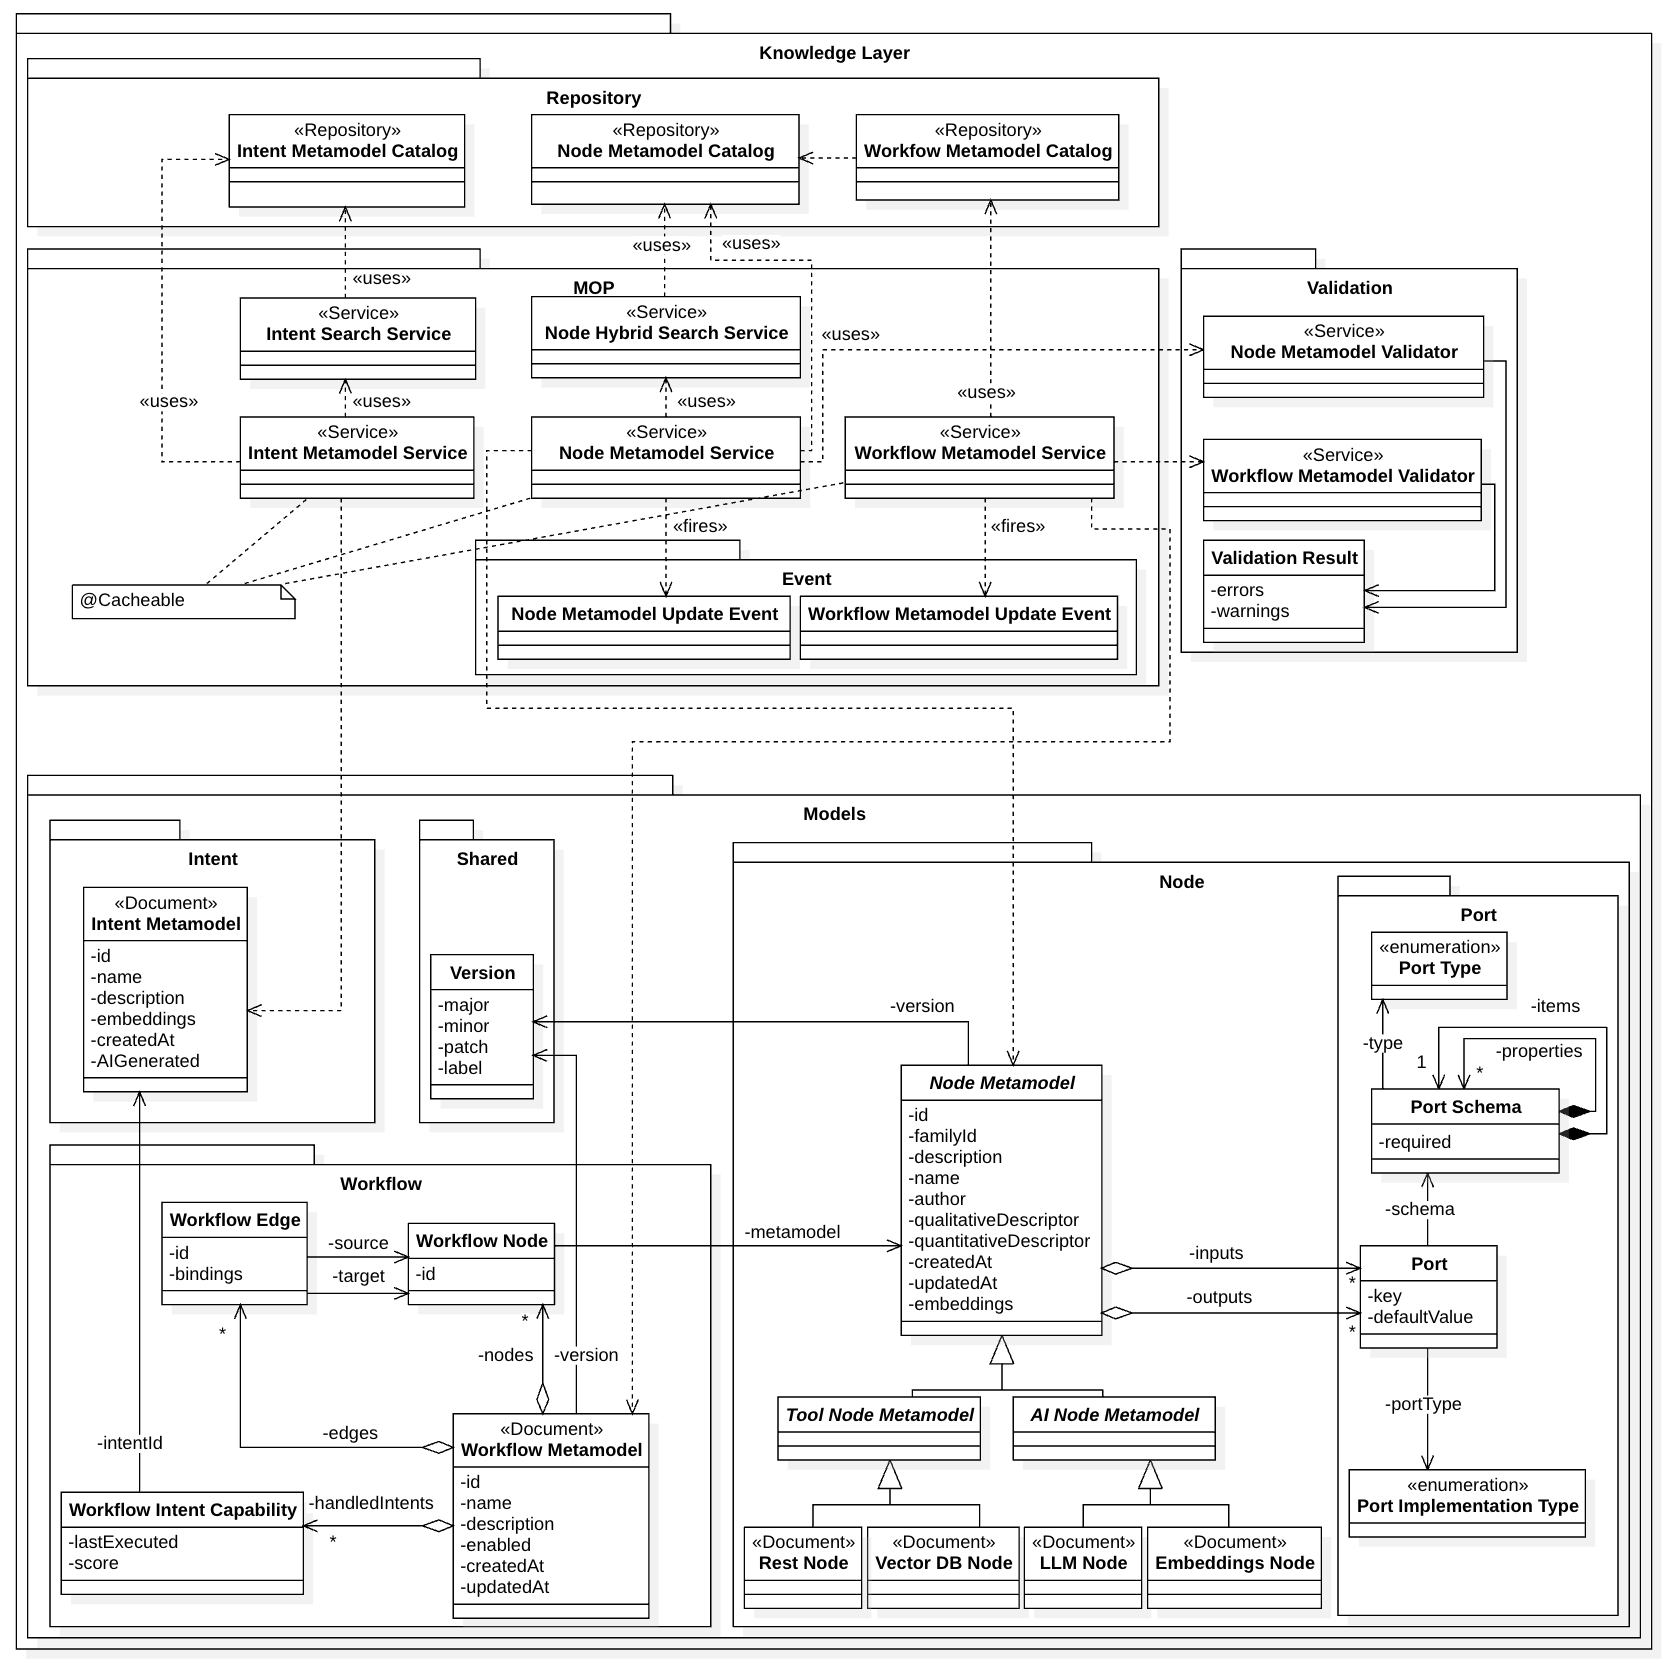
\includegraphics[width=1.2\textwidth]{Template_tesi/img/uml_knowledge.png}
  \end{adjustbox}
    \caption{UML Diagram of the \texttt{knowledge} package, illustrating its internal structure and relationships with other components. For conciseness, standard getters/setters and non-essential elements have been excluded.}
    \label{fig:uml_knowledge}
\end{figure}


\begin{figure}
  \centering
  \begin{adjustbox}{center}
    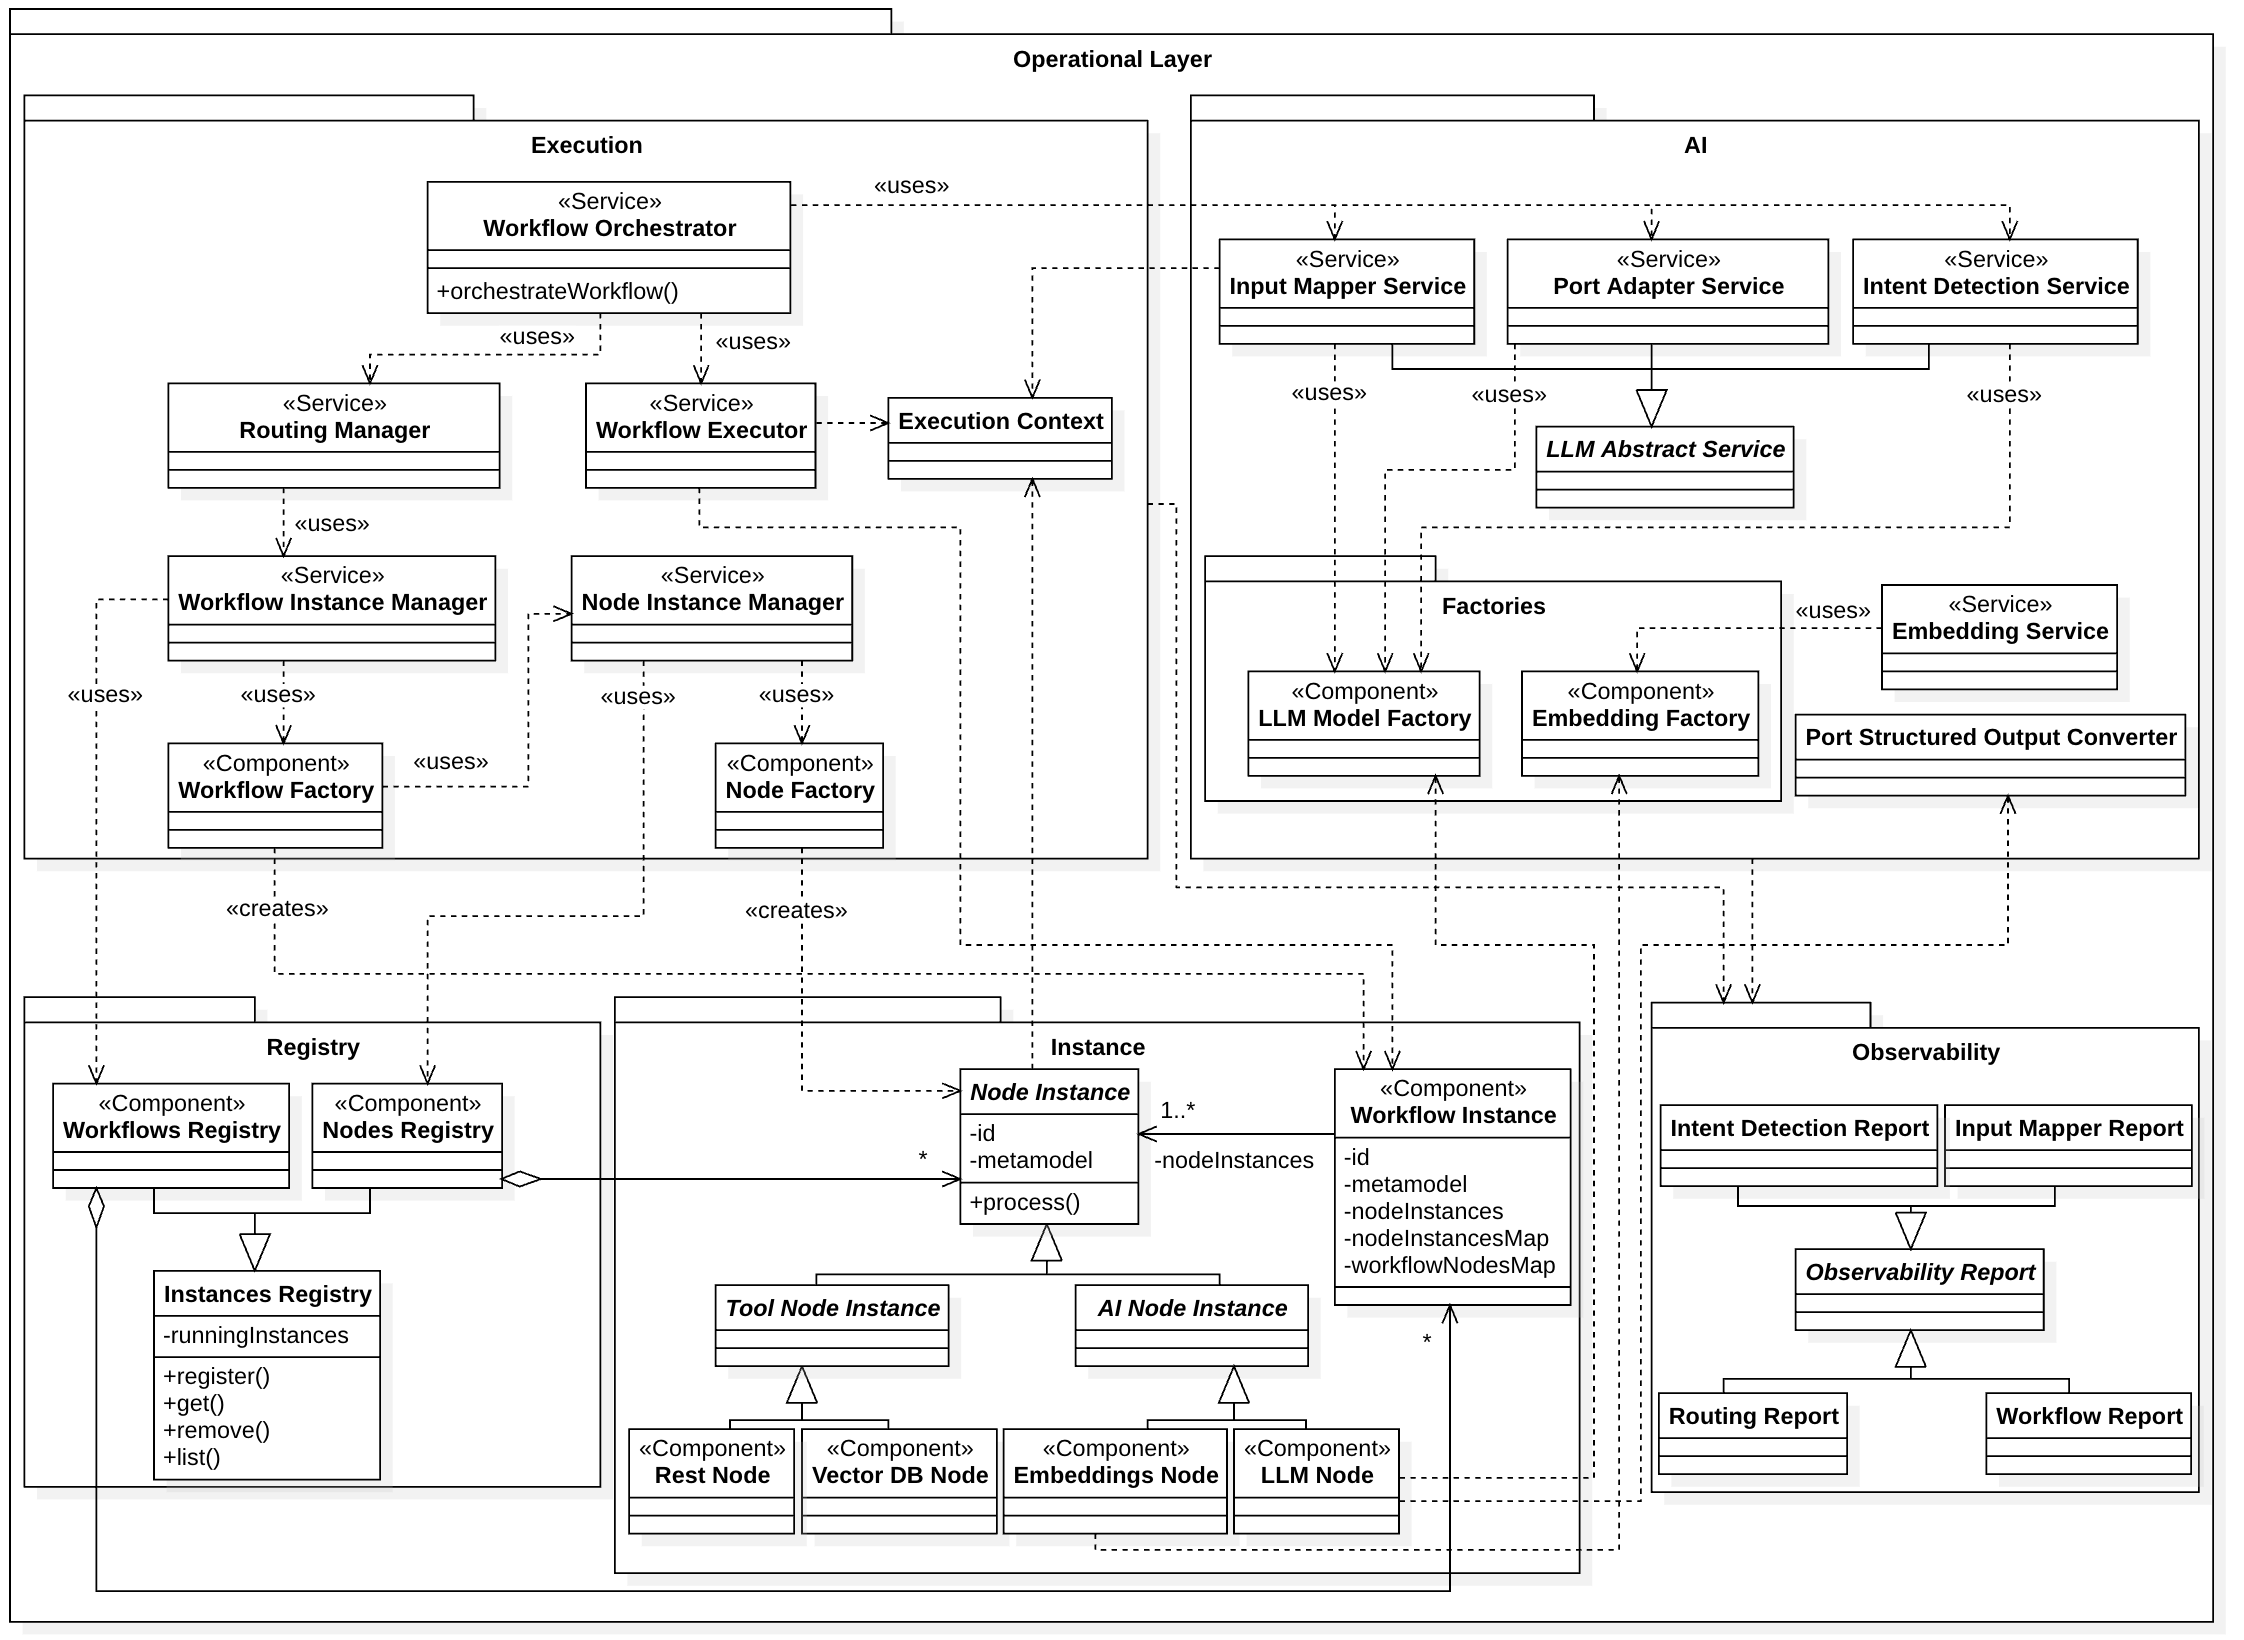
\includegraphics[width=1.2\textwidth]{Template_tesi/img/uml_operational.png}
  \end{adjustbox}
\caption{UML Diagram of the \texttt{Operational} package, presenting the core classes and their interactions within the operational layer. It details functionalities including workflow orchestration, AI services, instance management, and observability features. Standard getters/setters and non-essential elements are omitted for clarity.}
    \label{fig:uml_operational}
\end{figure}



Conversely, Figure~\ref{fig:uml_operational} illustrates the \textbf{Operational Layer}. This package includes the implementation of specialized workflow nodes that interact with external systems, such as databases, REST APIs, and AI service providers. Central to this layer is the \texttt{engine} package, which orchestrates the lifecycle of workflows—handling their retrieval, routing, and execution. Workflow and node instantiation are handled by specialized factory components, while two in-memory registries maintain records of active workflow and node instances, respectively. A significant component within the operational layer is the \texttt{AI} subpackage, which manages interactions with external providers of large language models and embedding services. It also exposes several essential LLM-powered services:

\begin{itemize}[leftmargin=*, label=--]
    \item \texttt{Input Mapper Service}: Translates user-provided request variables into the corresponding workflow inputs.
    
    \item \texttt{Port Adapter Service}: Resolves data-flow mismatches between workflow nodes.
    
    \item \texttt{Intent Detection Service}: Identifies and classifies the intent of the user.
\end{itemize}


\noindent
To enable dynamic and flexible model instantiation, a factory design pattern has been implemented. This allows LLM and embedding models to be initialized at runtime based on the specifications provided by the knowledge base. This approach encourages high configurability and supports seamless switching between different model providers, thus facilitating experimental evaluation and optimization.









\section*{AI Integration}

A central aspect of the system is the integration of large language models (LLMs) to enable cognitive workflows. For this purpose, Spring AI was selected as the primary framework (see Appendix \ref{ch:appendix_spring} for further details).
To evaluate both performance and system adaptability, multiple models and providers were tested across diverse services, demonstrating the flexibility offered by the model factories (see Figure \ref{fig:uml_operational}). Ultimately, \textbf{Claude 3.5 Sonnet} by Anthropic was selected for the \texttt{Input Mapper Service} and \texttt{Port Adaptation Service} due to its strong capabilities in schema handling, consistent structured outputs, and lower cost compared to more recent models like Claude 3.7 and Claude 4. For the \texttt{Intent Detector Service}, \textbf{GPT-4o} by OpenAI was integrated, providing state-of-the-art performance in intent classification. Finally, for generating embeddings, OpenAI’s \textbf{text-embedding-3-small} was employed to enable efficient vector search supporting intent classification.


\section*{Testing Summary}


The testing strategy covered unit, integration, and end-to-end tests, validating system correctness and robustness across 104 test cases:


\begin{itemize}[leftmargin=*, label=--]
    \item \textbf{Unit testing} involved 48 tests designed to verify the functionality of isolated components, such as metamodel validators and domain model methods.
    
    \item \textbf{Integration testing} included 54 tests that evaluated the interactions between components and services. LLM-based services were tested on real-world tasks spanning a wide range of scenarios, from simple to complex. Furthermore, the tests covered nodes that interact with external systems, such as database nodes and RESTful services, the latter simulated using WireMock\footnote{WireMock is an open-source tool for mocking HTTP-based APIs. See \url{https://wiremock.org}}.
    
    \item \textbf{End-to-end testing} involved two comprehensive tests simulating full workflow execution and adaptation in a production-like environment. These tests covered the entire process—from intent recognition to response generation—within the RAG scenario depicted in Figure~\ref{fig:RAG-workflow}.
\end{itemize}


A valuable insight from this testing regime is the role of integration tests that incorporate actual (non-mocked) LLM API calls. Although such tests incur considerable costs due to high API usage, they are essential for verifying system stability and functionality, particularly given the inherent non-deterministic nature of LLMs. By designing specific, nontrivial test cases that challenge the model's capabilities, this approach enables robust validation across different foundation models. It ensures resilience against potential regressions or failures resulting from model updates, optimizations, or changes in the underlying model provider.

It is important to note that, while database connections were mocked during the unit and integration testing phases to isolate system components, the end-to-end tests employed a dedicated MongoDB cluster. This environment was configured to closely replicate production conditions, providing a realistic scenario to validate the system's performance.


\subsection*{Test Coverage Report}
Table \ref{tab:code_coverage} presents the code coverage metrics of the implemented system.

\begin{table}[H]
\centering
\caption{Code coverage statistics by package.}
\label{tab:code_coverage}
\resizebox{\linewidth}{!}{%
\begin{tabular}{|l|c|c|c|}
\hline
\textbf{Package} & \textbf{Class Coverage} & \textbf{Method Coverage} & \textbf{Line Coverage} \\
\hline
\texttt{API} & 50\% (3/6) & 6\% (3/45) & 5\% (8/139) \\
\texttt{config} & 75\% (3/4) & 60\% (3/5) & 80\% (8/10) \\
\texttt{knowledge} & 88\% (55/62) & 73\% (244/333) & 63\% (902/1415) \\
\texttt{operational} & 77\% (51/66) & 71\% (236/332) & 75\% (1444/1906) \\

\hline
\textbf{Total (all packages)} & \textbf{80\% (112/139)} & \textbf{67\% (486/716)} & \textbf{68\% (2362/3471)} \\
\hline
\end{tabular}%
}
\end{table}






\section*{API Endpoints Overview}

The system exposes a RESTful API for manipulating the knowledge catalogs and performing requests. The following table summarizes the available endpoints, HTTP methods, and corresponding controllers.

\begin{table}[H]
\centering
\caption{Overview of exposed API endpoints and their respective controllers.}
\small
\begin{tabular}{|l|l|l|}
\hline
\textbf{Endpoint} & \textbf{Method} & \textbf{Controller} \\
\hline
\texttt{/api/workflows} & GET, POST & WorkflowController \\
\texttt{/api/workflows/execute} & POST & WorkflowController \\
\texttt{/api/workflows/\{id\}} & GET, PUT & WorkflowController \\
\hline
\texttt{/api/nodes} & GET, POST & NodeController \\
\texttt{/api/nodes/embeddings} & POST & NodeController \\
\texttt{/api/nodes/embeddings/\{id\}} & PUT & NodeController \\
\texttt{/api/nodes/gateway} & POST & NodeController \\
\texttt{/api/nodes/gateway/\{id\}} & PUT & NodeController \\
\texttt{/api/nodes/llm} & POST & NodeController \\
\texttt{/api/nodes/llm/\{id\}} & PUT & NodeController \\
\texttt{/api/nodes/rest-tool} & POST & NodeController \\
\texttt{/api/nodes/rest-tool/\{id\}} & PUT & NodeController \\
\texttt{/api/nodes/vector-db} & POST & NodeController \\
\texttt{/api/nodes/vector-db/\{id\}} & PUT & NodeController \\
\hline
\texttt{/api/intents} & GET, POST & IntentController \\
\texttt{/api/intents/\{id\}} & GET, PUT, DELETE & IntentController \\
\hline
\end{tabular}

\label{tab:api_endpoints}
\end{table}



\section*{Source Code Repository}
\noindent The complete source code is available at:
\begin{center}
\href{https://github.com/NiccoloCase/bsc-multi-agent-ai-framework}{\texttt{github.com/NiccoloCase/bsc-multi-agent-ai-framework}}
\end{center}

\noindent A permanent archive is accessible via DOI:
\begin{center}
\href{https://doi.org/10.5281/zenodo.15723912}{\texttt{doi.org/10.5281/zenodo.15723912}}
\end{center}

\noindent The repository contains all implementation files, documentation, and instructions necessary to reproduce the results described in this thesis.